\section{Motorstyring og bremsning}
For at finde den bedste måde at bremse på, er der lavet en test med tre scenarier. I alle tre scenarier er banen den samme. Banen består af 10 skinner. De første seks er tilsluttet strømforsyningen, mens de fire sidste er tilsluttet en kontakt så skinnerne kan frakobles strømforsyningen, kortsluttes eller strømmen vendes. Motoren er koblet direkte til banen, dvs. at den styres vha. strømforsyningen. I alle test er spændingsfaldet over motoren på 15 volt. Det hele filmes med højhastighedskamera. \\

I første test var de sidste fire skinner ikke tilsluttet til strømforsyningen ydermere var de ikke kortsluttet. Her viste testen at bilen skulle bruge mere en 70 cm. for at stoppe helt. \\
I anden test var de sidste fire skinner kortsluttet. Dvs. at motoren blev kortsluttet efter at have kørt på de seks første skinner. Her var bremselængden 67 cm. \\
I tredje test og sidste test løb strømmen den modsatte vej igennem motoren på de sidste fire skinner. Her var en væsentlig kortere bremselængde på kun 32 cm. \\

For at kunne vende strømmen i motoren er der placeret en h-bro. H-broen der anvendes er l293. Denne ic består af to h-broer, det er dog kun den ene som anvendes. H-broen er koblet til micro-controlleren med tre forbindelser. De tre forbindelser er enable, 1A og 2A. 

\begin{figure}[h!]
\center
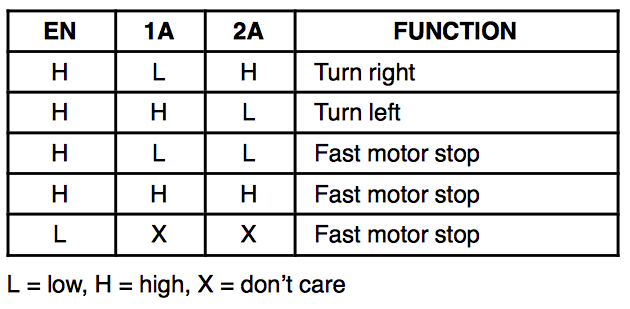
\includegraphics[scale=0.35]{./Graphics/h-bro_forbindelse.png}
\caption{H-broens 3 forbindelser og hvordan de kan sættes}
\label{hbro_forbindelse}
\end{figure}

PWM signalet fra micro-controlleren er koblet til 1A, mens enable og 2A er koblet til almindelige i/o pins. Som det ses vil et PWM signal medføre at motoren skifter mellem Fast motor stop og turn left. Dette er dog ikke et problem da man på lige strækninger kører med 100\% PWM hvilket svarer til at 1A konstant er høj. Derfor får man ikke lavere topfart i forhold til at køre uden h-bro. Dog vil det kræve et højere PWM signal for at holde samme fart i svingene i forhold til uden at bruge H-broen. Dette medvirker at bilen har et højere energiforbrug og mere spild energi, men der er intet krav om at bilen skal være effektiv. \todo{Skal dette med?} \\

Ved opbremsning ”slukkes” for PWM signalet og 2A sættes høj. Dette medfører at motoren prøver at køre den modsatte vej. Dette gøres kun kortvarigt så bilen kommer ned i en hastighed som gør at den ikke falder af i svingene. For at finde det optimale tidspunkt at bremse på er der lavet en række test og beregninger. Dette kan der læses nærmere om i afsnit \todo{afsnit udfyldes}.
